% Do Latent Volatility Regimes Improve Risk-Based Asset Allocation?
% Every number comes from paper/macros.tex, generated by
% scripts/generate_paper_outputs.py. No result is typed by hand.
\documentclass[11pt,letterpaper]{article}

\usepackage[margin=1.1in]{geometry}
\usepackage{amsmath,amssymb}
\usepackage{booktabs}
\usepackage{graphicx}
\usepackage{natbib}
\usepackage{caption}
% Must precede hyperref. Without hyphen breaking the repository URL in
% the availability declaration cannot wrap and runs 18.7pt into the
% margin, which the build gate rejects.
\usepackage[hyphens]{url}
\usepackage[hidelinks]{hyperref}
\usepackage{setspace}

\bibliographystyle{plainnat}
\captionsetup{font=small,labelfont=bf}
\onehalfspacing

% Generated by scripts/generate_paper_outputs.py. Do not edit.
% Manuscript release date: 2026-08-17

\newcommand{\releaseDate}{August 17, 2026}
\newcommand{\primarySharpeDiff}{0.021}
\newcommand{\primaryCiLower}{\ensuremath{-}0.075}
\newcommand{\primaryCiUpper}{0.115}
\newcommand{\primaryPValue}{0.327}
\newcommand{\primaryBootstrapSd}{0.048}
\newcommand{\primarySdsFromZero}{0.437}
\newcommand{\ciWidthMultiple}{9.0}
\newcommand{\blockMaxDeviation}{0.005}
\newcommand{\volDifference}{\ensuremath{-}0.175\,pp}
\newcommand{\volDifferenceMagnitude}{0.175\,pp}
\newcommand{\volCiLower}{\ensuremath{-}0.327\,pp}
\newcommand{\volCiUpper}{\ensuremath{-}0.033\,pp}
\newcommand{\hacAnnualReturnDiff}{0.314\,bps}
\newcommand{\hacStandardError}{36.216\,bps}
\newcommand{\hacPValue}{0.993}
\newcommand{\hacSdsFromZero}{0.009}
\newcommand{\equalWeightSharpe}{0.857}
\newcommand{\staticMinvarSharpe}{0.910}
\newcommand{\ewmaScaledSharpe}{0.945}
\newcommand{\regimeSharpe}{0.929}
\newcommand{\comparatorSharpe}{0.908}
\newcommand{\diffAtZeroBps}{0.031}
\newcommand{\diffAtTwentyBps}{0.011}
\newcommand{\regimeHalfTurnover}{54.19\%}
\newcommand{\comparatorHalfTurnover}{16.94\%}
\newcommand{\regimeCost}{10.838\,bps}
\newcommand{\comparatorCost}{3.388\,bps}
\newcommand{\turnoverRatio}{3.2}
\newcommand{\costHurdle}{7.450\,bps}
\newcommand{\threeStateDiff}{\ensuremath{-}0.028}
\newcommand{\dropRvDiff}{\ensuremath{-}0.023}
\newcommand{\capThirtyDiff}{0.050}
\newcommand{\capThirtyP}{0.011}
\newcommand{\capThirtyPHolm}{0.133}
\newcommand{\altSeedsDiff}{0.020}
\newcommand{\aTwoAcceptDiff}{0.018}
\newcommand{\kappaMaxMove}{0.002}
\newcommand{\capThirtyTotalChange}{0.029}
\newcommand{\capThirtyCostComponent}{0.008}
\newcommand{\capThirtyGrossComponent}{0.022}
\newcommand{\capThirtyCostShare}{26.6\%}
\newcommand{\capThirtyGrossShare}{73.4\%}
\newcommand{\nSpecsPositive}{11}
\newcommand{\nSignReversals}{2}
\newcommand{\nSpecsContainingZero}{12}
\newcommand{\nSecondaryMetrics}{5}
\newcommand{\nSecondaryExcludingZero}{1}
\newcommand{\nForecastPairsSurvivingHolm}{1}
\newcommand{\preTwentyTwentyDiff}{0.105}
\newcommand{\postTwentyTwentyDiff}{\ensuremath{-}0.076}
\newcommand{\covidDays}{232}
\newcommand{\tighteningDays}{460}
\newcommand{\oosYears}{16.6}
\newcommand{\ewmaMeanCondition}{116}
\newcommand{\ewmaMaxCondition}{505}
\newcommand{\stateOneCondition}{61.4}
\newcommand{\stateZeroCondition}{36.8}
\newcommand{\betweenStateMax}{0.16\%}
\newcommand{\threeStateMidOccupancy}{45.4\%}
\newcommand{\threeStateMinNeff}{487}
\newcommand{\equityCorrMin}{0.82}
\newcommand{\equityCorrMax}{0.92}
\newcommand{\aTwoFallbackOrigins}{4}
\newcommand{\argmaxToleranceDisagreements}{144}
\newcommand{\refitSeedChanges}{152}
\newcommand{\reproductionMaxDifference}{\ensuremath{1.45 \times 10^{-11}}}
\newcommand{\reproductionSeedDisagreements}{0}


\title{Does Regime Conditioning Improve Volatility-Aware Asset
Allocation?\\[0.3em]
\large A Prospectively Specified Walk-Forward Evaluation}
\author{Shakhrukh Kakhramonov\thanks{%
Zicklin School of Business, Baruch College, City University of New York,
New York, NY, USA.
ORCID: \orcidID{}.
Corresponding author: \correspondingEmail{}.
Code, analysis plan and complete output:
\url{https://github.com/kakhramonovsh-prog/regime-aware-asset-allocation}.
I thank the reviewers who read successive drafts of the design and
forced several corrections recorded in the amendment log.}}
% Never \today: it would change page 1, and therefore the PDF hash the
% visual inspection attests to, on every rebuild. Frozen in
% config/config.yaml (manuscript.release_date) and emitted as a macro.
\date{\releaseDate}

\begin{document}
\maketitle

% =====================================================================
% ABSTRACT — written last, inserted first
% =====================================================================
\begin{abstract}
\noindent
Between 2010 and 2026 I ran a minimum-variance portfolio of five US
exchange-traded funds that conditioned its covariance forecast on
volatility states inferred in real time from a two-state Gaussian hidden
Markov model, and compared it against the identical portfolio without
regime conditioning. Net of 10 basis points in transaction costs, the
regime-aware strategy earned an annualized Sharpe ratio
\primarySharpeDiff{} higher; the 95\% stationary-bootstrap interval runs
from \primaryCiLower{} to \primaryCiUpper{}, and the annualized return
difference is \hacAnnualReturnDiff{}. Regime conditioning lowered
annualized volatility by \volDifferenceMagnitude{}, but required
\turnoverRatio{} times the turnover, and the estimate falls from
\diffAtZeroBps{} to \diffAtTwentyBps{} as costs rise from
zero to 20 basis points. Across thirteen prespecified robustness
specifications the sign reverses twice and no comparison survives
multiplicity adjustment; portfolio constraints affected apparent
performance more than any modelling choice examined. The hypothesis,
sample split and robustness grid were fixed before estimation.
\end{abstract}

\vspace{0.5em}
\noindent\textbf{Keywords:} regime switching, hidden Markov models,
minimum-variance portfolios, out-of-sample evaluation, prospective specification,
transaction costs

\vspace{0.3em}
\noindent\textbf{JEL:} G11, G17, C58

% =====================================================================
\section{Introduction}
\label{sec:introduction}

A minimum-variance portfolio of five US exchange-traded funds that
conditioned its covariance forecast on volatility states inferred in
real time earned an annualized Sharpe ratio \primarySharpeDiff{} higher
than the same portfolio without regime conditioning over 2010--2026, net
of 10 basis points in transaction costs. The 95\% confidence interval on
that difference runs from \primaryCiLower{} to \primaryCiUpper{}. The
strategy did what the theory predicts, realizing \volDifferenceMagnitude{}
lower annualized volatility, but it traded \turnoverRatio{} times as much
as its comparator, and the estimated advantage falls monotonically as costs
rise. On this evidence, regime conditioning delivers a measurable risk
reduction too small relative to sampling variation to establish a
risk-adjusted improvement once trading costs are paid.

The design was fixed before the data were touched. I published the
hypothesis, the comparator, the sample split, the cost convention and
all thirteen robustness specifications, and version-tagged them in a
public repository before estimating a single model. Four later
amendments each carry a date and a record of what was known when I made
them; three were adopted before any portfolio return existed. The
comparison reported here is the one committed to in advance, not the one
that survived a search. Preregistration, frozen data, causal tests,
automated validation and dated amendments substantially constrained
ex-post researcher discretion, though they did not eliminate it.

The choice of comparator does most of the analytical work. Regime-aware
minimum variance beats equal weight and 60/40 comfortably on realized
Sharpe, and a study could stop there and report an improvement. It
should not. Those benchmarks differ from the regime strategy in
optimization, covariance estimation and regime conditioning at the same
time, so a gap between them attributes nothing to any single ingredient.
I therefore compare against rolling Ledoit--Wolf minimum variance, which
shares every ingredient except the regime signal. The \primarySharpeDiff{}
difference measures what regime conditioning adds on top of dynamic
covariance estimation, and it is not distinguishable from zero.

Three findings temper the point estimate further. The sign reverses
under a three-state specification and when realized volatility is
dropped from the feature set. It reverses again between the pre- and
post-2020 halves of the sample. And after Holm adjustment across the
robustness family, no specification retains significance. Set against
these, a positive point estimate with an interval \ciWidthMultiple{} times
its width is best read as inconclusive about small effects rather than as evidence
of either a benefit or its absence.

This paper contributes in three ways. It tests a regime-conditioning
strategy under a preregistered design with a matched comparator, which
is uncommon in the backtesting literature and directly addresses the
multiple-testing critique. It reports the full ablation ladder, showing
where risk-adjusted gains actually arise: mostly from optimization
itself rather than from dynamic covariance or regime conditioning. And
it documents an interaction the design did not anticipate, in which
portfolio constraints moved the estimated difference more than any
modelling choice examined.

\section{Related literature}
\label{sec:literature}

Three strands bear directly on this study.

\citet{hamilton1989} introduced the regime-switching framework this
paper applies, and with it the discipline that states are latent and
inferred rather than observed. That distinction governs the empirical
design here: the trading signal is the filtered probability at the
decision date, never a smoothed path that conditions on data the
investor did not have. The volatility clustering the framework describes
was documented by \citet{engle1982} and generalized by
\citet{bollerslev1986}; this paper does not revisit it, asking instead
whether acting on it survives out-of-sample testing net of costs.

Applying regime switching to allocation has a substantial literature.
\citet{ang2002} document regime shifts in international equity
correlations and their allocation consequences, \citet{guidolin2007}
solve multivariate regime-switching allocation problems, and
\citet{ang2012} survey the field. This paper's contribution is narrower
and more sceptical than a survey of that work would suggest: it holds
three things fixed at once --- states inferred strictly in real time, a
comparator differing by the regime signal alone, and trading costs
charged on realized turnover --- and preregisters the comparison before
estimating anything. The question is not whether regimes exist or
whether conditioning on them helps in principle, but what the
conditioning is worth after those three constraints are imposed
simultaneously.

\citet{demiguel2009} provide the closest methodological precedent. They
evaluate fourteen portfolio models across seven datasets and find that
none consistently outperforms naive 1/N allocation on Sharpe ratio,
certainty-equivalent return or turnover, concluding that estimation
error more than offsets the theoretical gain from optimization. Their
framing is the model for this study: a negative out-of-sample result
becomes informative when it identifies the mechanism by which a
theoretically superior method fails. The question here is one rung
further along --- optimization is granted, and the test is whether
regime conditioning adds anything on top of it.

\citet{harvey2015} and \citet{harvey2016} supply the inferential
standard. Documenting that hundreds of factors have been tested in the
cross-sectional literature, they argue that conventional significance
thresholds no longer establish anything and propose haircuts for
reported Sharpe ratios that account for the number of trials.
Preregistering a single primary comparison and applying Holm adjustment
across an explicitly bounded robustness family is a direct response to
that critique: the number of trials is fixed and published in advance
rather than reconstructed afterward.

The portfolio problem is \citet{markowitz1952} with the mean removed.
\citet{michaud1989} sets out why sample mean-variance optimization
performs poorly out of sample, which is the reason no strategy here uses
expected-return forecasts, and \citet{clarke2011} characterize what
minimum-variance portfolios actually hold. \citet{jagannathan2003} show
that imposing constraints which are wrong as beliefs can nonetheless
reduce estimation error and improve realized risk --- a result that
bears directly on the constraint interaction reported in
Section~\ref{sec:robustness}.

On methods, the covariance estimator follows \citet{ledoit2004}, whose
shrinkage approach is designed for exactly the near-collinear setting
observed here, where the equity block carries pairwise correlations
between \equityCorrMin{} and \equityCorrMax{}. The hidden Markov model is estimated by the EM
algorithm of \citet{dempster1977}. Volatility forecast evaluation uses
QLIKE following \citet{patton2011}, who shows that rankings can be
distorted when noisy volatility proxies are evaluated under
inappropriate loss functions, with pairwise comparisons following
\citet{diebold1995}. Inference uses the stationary bootstrap of
\citet{politis1994}, chosen because portfolio returns are serially
dependent and independent resampling would understate uncertainty;
\citet{ledoit2008} develop the robust Sharpe-ratio test that motivates
bootstrapping the difference rather than comparing ratios directly.
Standard errors on mean differences use \citet{newey1987}, and
multiplicity is handled by \citet{holm1979}. \citet{bailey2014} give
the sharpest statement of why backtested performance requires this kind
of discipline.


% =====================================================================
\section{Data and information availability}
\label{sec:data}

The universe is five liquid US-listed exchange-traded funds spanning
equities, duration and gold: SPY, QQQ, IWM, IEF and GLD. Daily adjusted
closes come from Yahoo Finance and proxy total returns. The sample
starts at GLD's inception on 18 November 2004, the binding constraint,
and ends 6 August 2026, giving 5{,}462 trading days.

Four macroeconomic series come from the St.\ Louis Fed's FRED database:
the CBOE Volatility Index (VIXCLS), 2- and 10-year Treasury constant
maturity yields (DGS2, DGS10) and the effective federal funds rate
(DFF). I use DFF rather than FEDFUNDS because the former is daily and
the latter a monthly average. The yield-curve slope is constructed
explicitly as DGS10 minus DGS2 rather than taken from the published
T10Y2Y series, which I retain only as a cross-check.

\paragraph{Alignment and missing values.} The asset panel keeps only
dates on which all five funds print an adjusted close. Macro series are
reindexed to those trading days and forward-filled by at most five
trading days; a longer gap raises an error rather than propagating a
stale value. Backward filling is never used, so values before a series
begins remain missing and are reported as such. Two calendar gaps
longer than four days survive in the sample, both genuine exchange
closures: the day of mourning for President Ford in January 2007 and
Hurricane Sandy in October 2012.

\paragraph{Information availability.} All FRED-sourced series enter
signals with an additional one-trading-day lag, because H.15 yields are
published with a lag and same-close availability of the VIX print is not
guaranteed for a close-of-day decision. Price-derived features use
information through the close of date $t$ without extra lag. This policy
is fixed for every specification.

\paragraph{Data licensing.} Neither vendor permits redistribution of the
raw series: Yahoo grants a personal, non-transferable licence, and
VIXCLS carries a CBOE copyright requiring the owner's permission for
non-personal use. The repository therefore publishes SHA-256 hashes and
full metadata for every raw file, the download scripts, every generated
table and figure, and per-phase provenance manifests, but no vendor
data. A reader can audit every computation without receiving a byte of
licensed data.

% =====================================================================
\section{Prospectively specified empirical design}
\label{sec:design}

The hypothesis, comparator, sample split, cost convention and complete
robustness grid were fixed and version-tagged before any model was
estimated. Four amendments followed, each dated and each recording what
was known when it was made; three were adopted before any portfolio
return existed.

The analysis plan was time-stamped in a private version-controlled
repository before model estimation rather than lodged with a public
registry, so this study is described as prospectively specified rather
than preregistered. The original development history is preserved and
can be provided confidentially to editors or reviewers.

\paragraph{Hypothesis.} The primary null is
\begin{equation}
H_0:\quad SR^{\text{net}}_{\text{regime}} -
SR^{\text{net}}_{\text{rolling LW}} \le 0,
\end{equation}
tested net of 10 basis points in transaction costs. The comparator is
deliberately the \emph{closest non-regime strategy}, not equal weight or
60/40. Those naive benchmarks differ from the regime strategy in
optimization, covariance estimation and regime conditioning
simultaneously, so a gap between them would attribute nothing. Rolling
Ledoit--Wolf minimum variance shares every ingredient except the regime
signal, which isolates what regime conditioning adds.

\paragraph{Sample split.} The initial training window runs from
18 November 2004 to 31 December 2009. The out-of-sample period begins
1 January 2010 and ends 6 August 2026. The first signal is formed at the
December 2009 month-end close and executed on 4 January 2010, giving 200
monthly rebalancing decisions.

\paragraph{Information and execution timeline.} At each month-end $t$:
information is observed through the close of $t$; all models are
estimated using data through $t$ only; target weights are computed;
trades execute at the close of the \emph{next} trading day $t+1$; and
the new weights first earn the $t{+}1 \to t{+}2$ return. Because the
dataset contains adjusted closes only, assuming execution at the same
close where the signal was observed would constitute look-ahead. The
convention costs one day of exposure and removes the ambiguity.

\paragraph{Look-ahead controls.} A truncation test verifies that no
derived quantity changes when future data is removed: for any date $t$,
perturbing or deleting observations after $t$ must leave every value
dated $t$ or earlier bit-identical. The test is applied to feature
construction, volatility forecasts, covariance estimates and the full
accounting layer.

\paragraph{Strategy ladder.} Six strategies form an ablation ladder in
which each rung adds exactly one ingredient:
equal weight; 60/40 SPY/IEF; static minimum variance estimated once on
the training window; rolling Ledoit--Wolf minimum variance;
volatility-scaled minimum variance using EWMA variance forecasts with
Ledoit--Wolf correlations; and regime-aware minimum variance. Reading performance
down the ladder attributes any improvement to dynamic covariance,
volatility forecasting or regime conditioning specifically.

Optimized strategies are long only, fully invested, and capped at 40\%
per asset, solved by sequential quadratic programming. The 60/40
benchmark is exempt from the cap by construction, since it deliberately
holds 60\% SPY. No strategy uses expected-return forecasts.

\paragraph{Costs.} Turnover compares new targets against pre-trade
holdings \emph{drifted} by realized returns since the last rebalance,
with the drift recurrence applied every trading day. Costs are charged
on the full traded notional $\sum_i |w^{\text{target}}_i -
w^{\text{pre}}_i|$; the halved figure is used only for reporting.
Returns compound multiplicatively,
\begin{equation}
1 + r^{\text{net}}_t = \left(1 + r^{\text{gross}}_t\right)
\left(1 - c \sum_i \left| w^{\text{target}}_{i,t} -
w^{\text{pre}}_{i,t} \right| \right),
\end{equation}
rather than by subtracting cost from return. Every strategy begins from
100\% cash at the first execution, so all six pay an identical entry
cost on a traded notional of one.

% =====================================================================
\section{Volatility and regime estimation}
\label{sec:estimation}

\paragraph{Volatility.} Three forecasts are compared out of sample:
63-day rolling historical variance, EWMA with $\lambda = 0.94$, and
GARCH(1,1) with normal innovations refit at every rebalance date. The
forecast target is the integrated variance over the next holding period,
evaluated by QLIKE as the primary loss. GARCH attains the lowest QLIKE
for all five assets, but only \nForecastPairsSurvivingHolm{} of the
fifteen pairwise comparisons survives Holm adjustment at the 5\%
level. EWMA was fixed
\emph{ex ante} as the model feeding the portfolio, so this comparison
does not and cannot promote GARCH into the main specification; a
GARCH-fed variant belongs to robustness.

\paragraph{Regimes.} A two-state Gaussian hidden Markov model is refit at
every rebalance date on an expanding window, using four standardized
features: SPY log return, 21-day realized volatility, one-day-lagged log
VIX and one-day-lagged yield-curve slope. Standardization uses the
estimation window only.

The trading signal is the \emph{filtered} probability
$p_t = P(S_t = k \mid \mathcal{F}_t)$, taken as the posterior at the
final observation of the sample truncated at $t$, where forward
filtering and forward--backward smoothing coincide because no
observation follows the endpoint. Full-sample smoothed paths are
computed separately, stored in their own file and used only for
descriptive figures; they never inform a trading decision.

Each refit runs sixteen predetermined initializations (seeds 42--57).
States are relabeled after every fit by ascending training-window mean
realized volatility, so state~0 is always the lower-volatility state; no
code path assumes the estimator's raw labels carry meaning. A refit
whose state occupancy falls below 5\%, whose state covariance is
singular, or whose transition matrix contains an absorbing row is
flagged degenerate.

% =====================================================================
\section{Covariance and portfolio construction}
\label{sec:covariance}

At each rebalance date the regime-conditioned covariance is built in
four steps. First, the filtered state probability $p_t$. Second,
horizon-averaged probabilities over the $H = 21$ day holding period,
$\bar{p}_t(H) = H^{-1}\sum_{h=1}^{H} p_t P_t^h$, using the transition
matrix estimated through $t$. Third, state-conditional covariances
$C_{k,t}$, computed as responsibility-weighted covariances around each
state's own mean and shrunk toward the unconditional Ledoit--Wolf
estimate with weight $\alpha_k = n_{\text{eff},k} /
(n_{\text{eff},k} + 60)$ on the state estimate, where
$n_{\text{eff},k} = (\sum_s \gamma_{s,k})^2 / \sum_s \gamma_{s,k}^2$.
Fourth, the mixture
\begin{equation}
\Sigma_{\text{RA},t} = \sum_k \bar{p}_{t,k}(H)\, C_{k,t}.
\label{eq:mixture}
\end{equation}

Equation~\eqref{eq:mixture} is a within-state mixture: it omits the
between-state mean-dispersion term and so treats conditional means as
common across states. That is a deliberate simplification consistent
with the design's prohibition on expected-return forecasting, and it is
documented as an assumption rather than presented as the complete law of
total covariance. Its magnitude is measured at every rebalance: the
omitted term reaches at most \betweenStateMax{} of the within-state
mixture and never exceeds 1\%. The complete formula is carried as a
robustness case.

Conditioning diagnostics motivate the shrinkage. Across 200 origins the
raw EWMA covariance is the worst-conditioned estimator, averaging a
condition number of \ewmaMeanCondition{} and peaking at
\ewmaMaxCondition{}, which is why the
volatility-scaled strategy combines EWMA variances with Ledoit--Wolf
correlations rather than using the EWMA covariance directly. The
high-volatility state is materially worse conditioned than the
low-volatility state (means of \stateOneCondition{} versus
\stateZeroCondition{}), so the stressed-state
matrix is nearest to singular exactly when a variance minimizer leans on
it hardest. No matrix in the panel required a positive-semidefinite
correction.

\paragraph{Degeneracy policy.} A degenerate fit keeps its probability,
which is reported unchanged, but does not supply a regime-conditioned
covariance for that rebalance; the allocation uses the unconditional
Ledoit--Wolf estimate instead, and the fallback is audit-logged.
\aTwoFallbackOrigins{} of
200 origins invoked this rule, all for absorbing transition rows. The
routing depends solely on the diagnostic flags; the affected dates are
audit information and appear in no routing condition.

% =====================================================================
\section{Primary results and inference}
\label{sec:results}

\subsection{Realized performance}

Table~\ref{tab:table1_performance} reports the six strategies over
2010--2026, net of 10 basis points. The regime-aware strategy earned a
Sharpe ratio of \regimeSharpe{} against the comparator's
\comparatorSharpe{}. Reading down the ladder, most of the risk-adjusted
gain over the naive benchmarks comes from optimization itself rather
than from anything dynamic: equal weight earns \equalWeightSharpe{} and
static minimum variance \staticMinvarSharpe{}, after which dynamic
covariance adds nothing measurable (\comparatorSharpe{}) and the two
responsive rungs add modest further amounts.

The highest realized Sharpe in the ladder belongs to the
volatility-scaled strategy (\ewmaScaledSharpe{}), not to the regime-aware strategy.
That was not predicted by the design and is reported as found; it does
not alter the preregistered hypothesis, which concerns the regime rung.

\begin{table}[htbp]
\caption{Realized performance, 2010--2026, net of 10 basis points. Annualized figures; maximum drawdown from the net wealth path.}
\label{tab:table1_performance}
\small
\begin{tabular}{lrrrrrr}
\toprule
 & CAGR (\%) & Volatility (\%) & Sharpe & Sortino & Max DD (\%) & Calmar \\
\midrule
Equal weight & 11.61 & 11.90 & 0.857 & 1.214 & $-$22.80 & 0.509 \\
60/40 & 9.82 & 9.78 & 0.852 & 1.207 & $-$21.20 & 0.463 \\
Static min-var & 9.04 & 8.23 & 0.910 & 1.301 & $-$19.17 & 0.471 \\
Rolling LW min-var & 8.71 & 7.88 & 0.908 & 1.293 & $-$17.41 & 0.500 \\
EWMA-scaled min-var & 8.70 & 7.54 & 0.945 & 1.356 & $-$17.30 & 0.503 \\
Regime-aware min-var & 8.73 & 7.71 & 0.929 & 1.331 & $-$17.44 & 0.501 \\
\bottomrule
\end{tabular}
\end{table}


\subsection{The preregistered comparison}

The estimated difference in annualized net Sharpe ratio between the
regime-aware strategy and rolling Ledoit--Wolf minimum variance is
\begin{equation}
\widehat{\Delta SR} = \primarySharpeDiff, \qquad
\text{95\% CI } [\primaryCiLower,\ \primaryCiUpper], \qquad
p = \primaryPValue .
\end{equation}

The interval is roughly \ciWidthMultiple{} times as wide as the point
estimate and contains zero comfortably; the estimate sits
\primarySdsFromZero{} bootstrap standard deviations from zero. $H_0$ is
not rejected.

Inference uses a stationary bootstrap with 10{,}000 replications, mean
block length 21 trading days and seed 12345, applied to \emph{paired
daily excess returns} annualized by $\sqrt{252}$ --- the same estimand
the point estimate reports. Both strategies receive identical bootstrap
indices in every replication, preserving contemporaneous pairing; a test
confirms that feeding the same series twice yields exactly zero
difference with zero variance. The one-sided $p$-value comes from the
centered null $\Delta SR_b - \widehat{\Delta SR}$, not from the fraction
of ordinary draws below zero, which is a different quantity.

The conclusion is insensitive to block length: mean blocks of 10, 42 and
63 days all produce interval bounds within \blockMaxDeviation{} of the
primary bounds, and every one contains zero.

\subsection{Returns and volatility separately}

Mean returns are indistinguishable. Paired daily net return differences
give an annualized arithmetic difference of \hacAnnualReturnDiff{}
against a Newey--West standard error of \hacStandardError{}, so the
estimate sits \hacSdsFromZero{} standard errors from zero
($p = \hacPValue{}$, HAC lag 21; lags of 5 and 42 give the same
conclusion).

Among the \nSecondaryMetrics{} secondary metric intervals, only
annualized volatility excludes zero: the regime-aware strategy's is
lower by \volDifferenceMagnitude{}, with a 95\% interval on that
difference running from \volCiLower{} to \volCiUpper{}. This is a secondary, unadjusted interval among several examined
metrics and is not confirmatory evidence. What raises it above an
incidental finding is that it is the outcome the mechanism predicts: a
variance minimizer given additional information about variance should
reduce variance. It is not described as statistically established.

\subsection{Trading costs}

The regime-aware strategy trades \regimeHalfTurnover{} annual
half-turnover against the comparator's \comparatorHalfTurnover{}, a
factor of \turnoverRatio{}. At the primary cost assumption it spends
\regimeCost{} per year against the comparator's \comparatorCost{}, a
hurdle of \costHurdle{} that its risk reduction must clear. The estimated
Sharpe advantage falls monotonically with costs, from \diffAtZeroBps{} at
zero to \diffAtTwentyBps{} at 20 basis points, and no cost level produces
an interval excluding zero.

\begin{table}[htbp]
\caption{Preregistered primary comparison. Paired stationary bootstrap, 10{,}000 replications, mean block 21 trading days, seed 12345, on daily excess returns.}
\label{tab:table2_primary_inference}
\small
\begin{tabular}{lrrrr}
\toprule
 & $\Delta$ Sharpe & CI lower & CI upper & p-value \\
\midrule
Regime-aware $-$ rolling LW & 0.021 & $-$0.075 & 0.115 & 0.327 \\
\bottomrule
\end{tabular}
\end{table}


\section{Robustness}
\label{sec:robustness}

Thirteen specifications each vary one factor at a time from the primary
model; no Cartesian product is constructed. Figure~\ref{fig:forest}
shows the Sharpe difference and its interval across all of them, ordered
as declared before any result was seen rather than sorted by effect.

\begin{figure}[htbp]
\centering
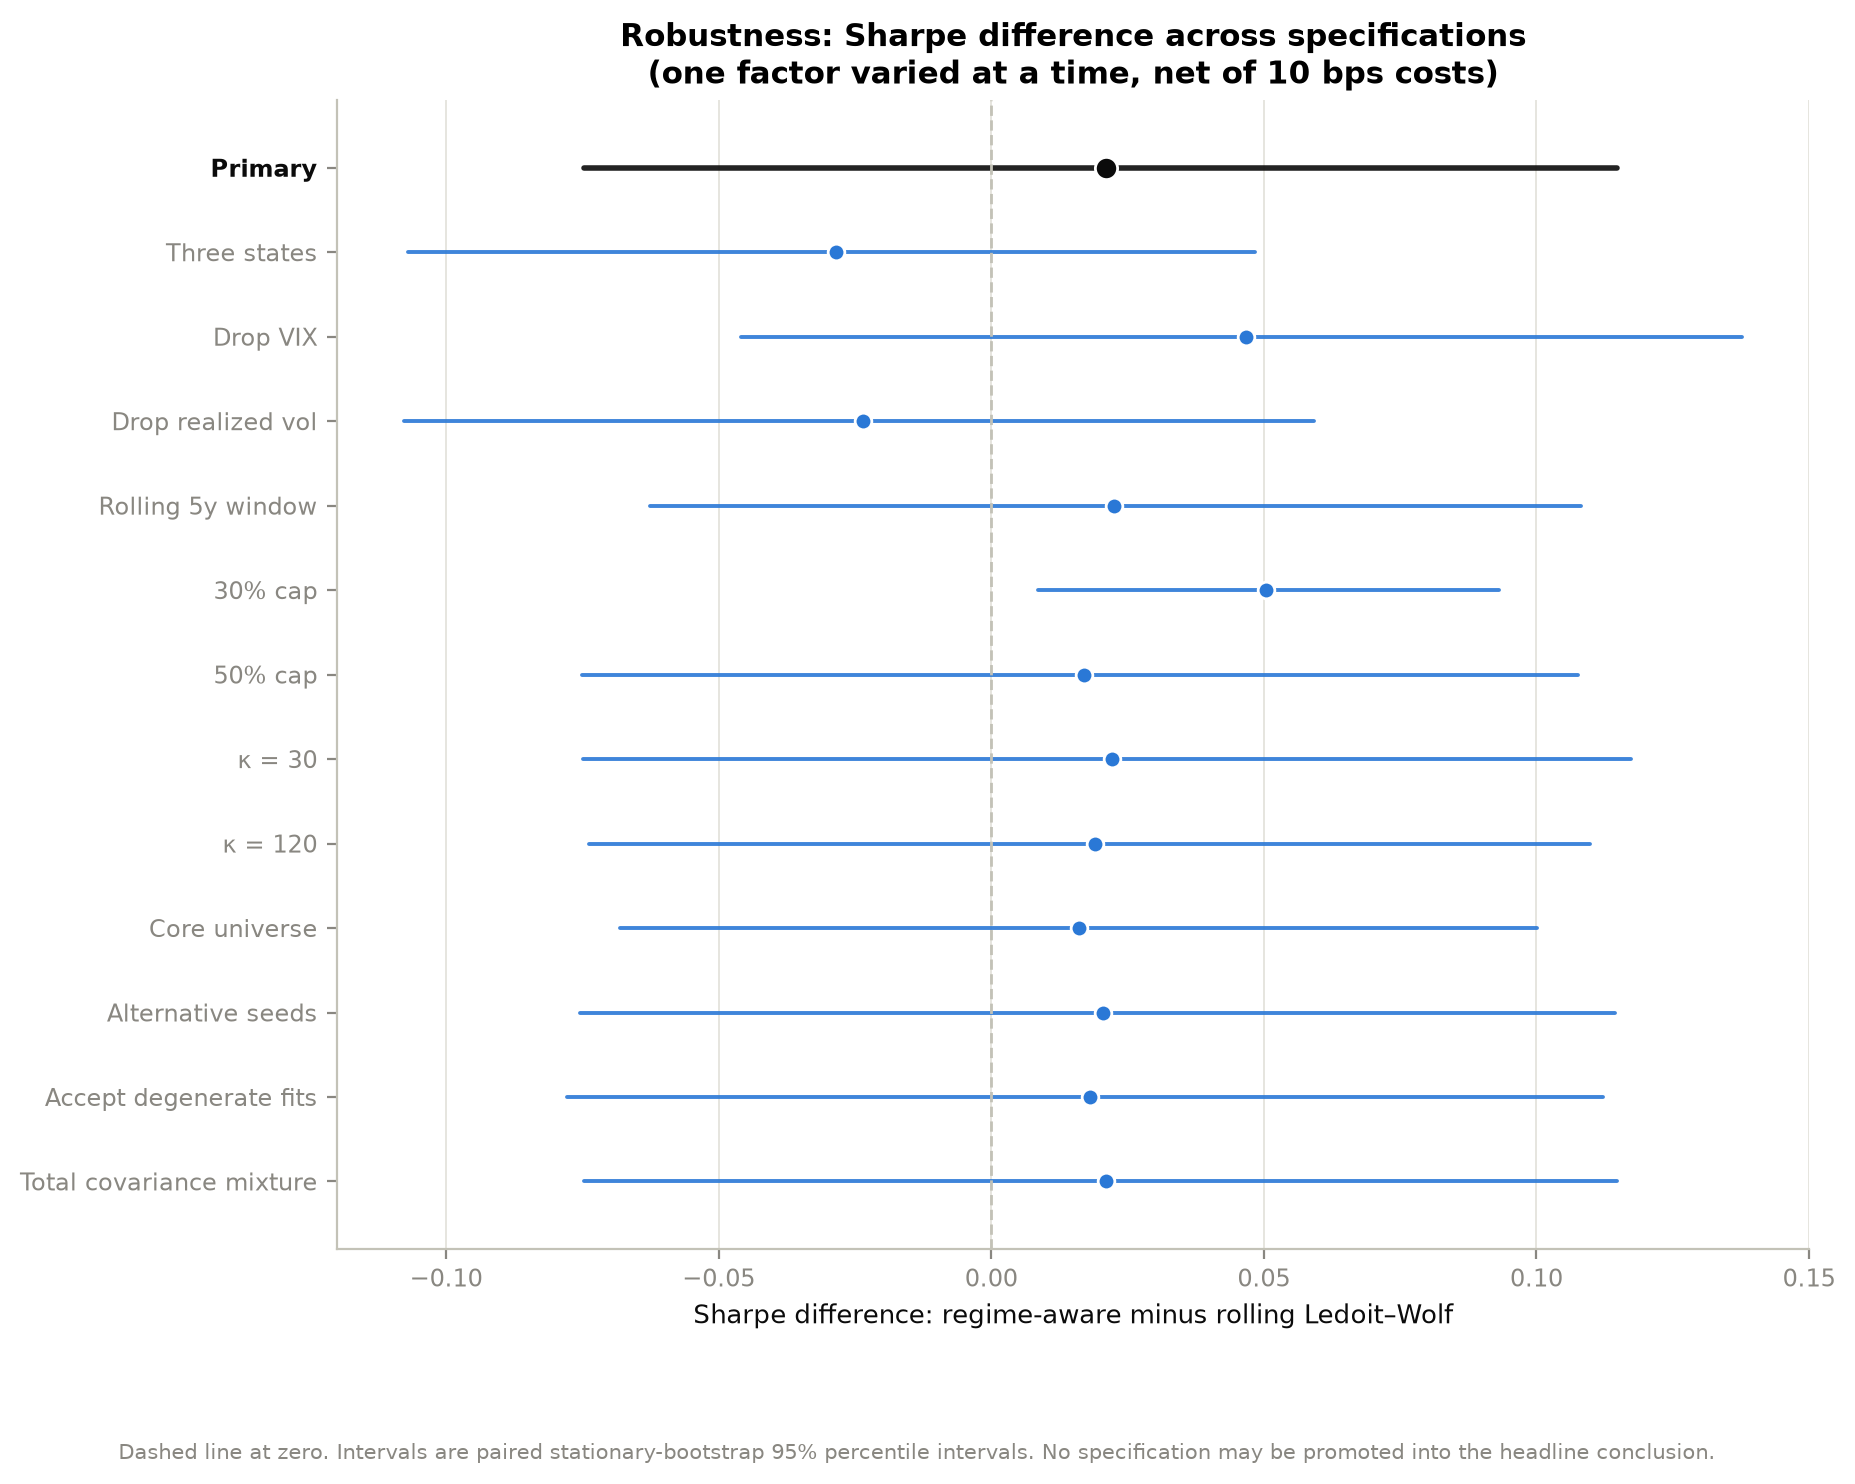
\includegraphics[width=\textwidth]{figures/robustness_forest.png}
\caption{Sharpe difference between the regime-aware strategy and rolling
Ledoit--Wolf minimum variance across thirteen specifications, each
varying one factor. Intervals are paired stationary-bootstrap 95\%
percentile intervals; the primary specification is shown in black. Only
the 30\% weight cap excludes zero, and it does not survive Holm
adjustment.}
\label{fig:forest}
\end{figure}

Point estimates are positive in \nSpecsPositive{} of the thirteen
specifications, and \nSpecsContainingZero{} of the thirteen intervals
contain zero. \textbf{After Holm adjustment across the
twelve-specification robustness family, nothing survives.}

\paragraph{Sign instability.} The estimate reverses sign in
\nSignReversals{} of the preregistered variations: the three-state HMM
(\threeStateDiff{}) and dropping realized
volatility from the feature set (\dropRvDiff{}). Neither reversal is
significant, but a result that changes direction when the state count
changes is fragile. The three-state model is not itself defective --- its
middle state holds \threeStateMidOccupancy{} occupancy with a minimum
effective sample size of \threeStateMinNeff{}, canonical
low--medium--high ordering holds at every refit, and no initialization
failed --- so the reversal reflects the estimate rather than a broken
fit.

\paragraph{The weight cap.} The 30\% cap is the only specification whose
unadjusted interval excludes zero (\capThirtyDiff{},
$p = \capThirtyP{}$), and it does not survive Holm adjustment
($p = \capThirtyPHolm{}$). Decomposing it exactly, using
$\Delta SR(\text{0 bps}) - \Delta SR(\text{10 bps})$ rather than
approximating cost expenditure divided by volatility: reduced cost drag
accounts for \capThirtyCostComponent{} of the \capThirtyTotalChange{}
change from the 40\% cap (\capThirtyCostShare{}), while gross pre-cost
differences account for \capThirtyGrossComponent{}
(\capThirtyGrossShare{}). Under the 30\% cap the volatility advantage disappears while
the relative turnover penalty falls substantially; however, reduced
transaction costs explain only part of the larger Sharpe difference,
with altered portfolio exposures and gross-return realizations
accounting for the remainder.

\paragraph{Factors that barely move the estimate.} The complete
total-covariance mixture reproduces the primary estimate to four
decimals, confirming the measured negligibility of the omitted
between-state term. Shrinkage thresholds of 30 and 120 move the estimate
by at most \kappaMaxMove{}. An alternative seed block gives
\altSeedsDiff{} against the primary \primarySharpeDiff{}, despite the
selected seed changing at \refitSeedChanges{} of 199 consecutive refits.
Accepting the degenerate fits rather than falling back gives
\aTwoAcceptDiff{}.

\paragraph{Subperiods.} Sliced descriptively from the primary paths, the
pre-2020 estimate is \preTwentyTwentyDiff{} and the post-2020 estimate is
\postTwentyTwentyDiff{}. With \covidDays{} days in the COVID slice and
\tighteningDays{} in the 2022 tightening slice,
these samples are far too small for inference, and the sign disagreement
between halves of the sample is a further reason for caution about the
full-sample point estimate. No subperiod is promoted.

\begin{table}[htbp]
\caption{Robustness grid: thirteen specifications, each varying one factor from the primary model.}
\label{tab:table4_robustness_grid}
\small
\begin{tabular}{lrrrr}
\toprule
 & $\Delta$ Sharpe & CI lower & CI upper & $\Delta$ Vol (pp) \\
\midrule
Primary & 0.021 & $-$0.075 & 0.115 & $-$0.175 \\
Three states & $-$0.028 & $-$0.107 & 0.048 & $-$0.180 \\
Drop VIX & 0.047 & $-$0.046 & 0.138 & $-$0.117 \\
Drop realized vol & $-$0.023 & $-$0.108 & 0.059 & $-$0.052 \\
Rolling 5y window & 0.022 & $-$0.063 & 0.108 & $-$0.206 \\
30\% cap & 0.050 & 0.009 & 0.093 & 0.033 \\
50\% cap & 0.017 & $-$0.075 & 0.108 & $-$0.137 \\
$\kappa$ = 30 & 0.022 & $-$0.075 & 0.117 & $-$0.175 \\
$\kappa$ = 120 & 0.019 & $-$0.074 & 0.110 & $-$0.177 \\
Core universe & 0.016 & $-$0.068 & 0.100 & $-$0.188 \\
Alternative seeds & 0.020 & $-$0.075 & 0.114 & $-$0.175 \\
Accept degenerate fits & 0.018 & $-$0.078 & 0.112 & $-$0.171 \\
Total covariance mixture & 0.021 & $-$0.075 & 0.115 & $-$0.175 \\
\bottomrule
\end{tabular}
\end{table}


\section{Limitations}
\label{sec:limitations}

\paragraph{Precision.} Despite approximately \oosYears{} years of out-of-sample
returns, the study had limited precision for detecting small differences
in risk-adjusted performance. The estimated Sharpe difference was
\primarySharpeDiff{}, while its 95\% bootstrap interval ranged from
\primaryCiLower{} to \primaryCiUpper{}. Consequently, the analysis
provides no confirmatory evidence of improvement, but it also cannot
exclude economically modest positive or negative effects. The results
should therefore be interpreted as inconclusive regarding small effects
rather than as evidence that regime conditioning has exactly zero value.

The binding constraint is information rather than raw observation count.
Inference uses daily paired returns, but the strategy makes only about
200 rebalancing decisions, and serial dependence in both returns and
regime states further reduces the effective information available to
distinguish two highly correlated strategies.

\paragraph{Universe selection.} Exchange-traded funds avoid single-name
survivorship bias, but choosing these five funds in 2026 uses knowledge
that they survived and remained liquid. All conclusions are conditional
on the universe.

\paragraph{Vendor data.} Yahoo adjusted closes are restated when
distributions occur, so the analysis is tied to a specific frozen
snapshot rather than to a canonical dataset. Cross-validation against
CRSP or a commercial vendor would strengthen it.

\paragraph{Cost model.} Costs are proportional to traded notional. The
model excludes market impact, taxes, borrowing constraints and bid--ask
dynamics, all of which would penalize the higher-turnover strategies
further.

\paragraph{Scope.} One market, one asset-class mix, one regime
specification family. Whether the finding extends to international
assets, credit, or intraday-informed volatility estimates is untested.

\paragraph{Numerical reproduction.} Two independent runs produced
filtered probabilities differing by up to \reproductionMaxDifference{},
while all selected seeds, classifications and reported conclusions
reproduced. Exact argmax selection and tolerance-based selection were
each stable across the two runs, although they selected different seeds
at \argmaxToleranceDisagreements{} of
200 origins. The evidence therefore supports numerical stability of both
rules but does not establish that the tolerance rule was necessary for
reproduction.

\paragraph{Researcher discretion.} Preregistration, frozen data, causal
tests, automated validation and dated amendments substantially
constrained ex-post researcher discretion. All amendments were
documented before viewing the results they could influence. Discretion
was constrained, not eliminated: implementation choices were made
throughout, and four amendments modified the frozen plan after it was
tagged.


\section{Discussion and conclusion}
\label{sec:conclusion}

Regime conditioning modestly reduced realized volatility in the primary
specification but did not produce statistically credible improvement in
net risk-adjusted performance. Results were sensitive to state
specification, feature selection, sample period, and portfolio
constraints.

The mechanism is visible even though the effect is not. Conditioning a
covariance forecast on an inferred volatility state does what theory
suggests: the regime-aware portfolio realized \volDifferenceMagnitude{}
lower annualized volatility than an otherwise identical strategy. The
difficulty is that this reduction is small relative to sampling
variation, and harvesting it required \turnoverRatio{} times the
turnover, which consumed \costHurdle{} per year more than its comparator.
What survives after costs is
\primarySharpeDiff{} in Sharpe ratio, with an interval that runs from
\primaryCiLower{} to \primaryCiUpper{}.

That pattern echoes \citet{demiguel2009}, who found that none of
fourteen optimization models consistently beat naive 1/N out of sample
because estimation error offsets the theoretical gain from
optimization. The result here sits one rung further up the same ladder:
optimization beats naive allocation in this sample, but adding regime
conditioning on top of dynamic covariance estimation does not produce a
detectable further gain. The obstacle in both cases is the gap between
what a model improves in principle and what survives estimation error
and trading frictions in practice.

Two features of the robustness evidence deserve weight in any reading of
the point estimate. The sign reverses under a three-state specification
and when realized volatility is dropped from the feature set, and it
reverses again between the pre- and post-2020 halves of the sample. A
result that changes direction under prespecified variations of this
kind is fragile regardless of its interval.

One observation the design did not set out to test deserves attention,
and equally deserves careful labelling. Tightening the weight cap from
40\% to 30\% changed the estimated difference by more than any modelling
choice examined, and decomposition attributes \capThirtyGrossShare{} of
that change to altered exposures and realized returns rather than to the
cost saving from reduced turnover. This is consistent with
\citet{jagannathan2003}, who show that constraints wrong as statements
of belief can still improve realized risk by suppressing estimation
error.

The status of that observation must be stated precisely, because it is
the result most likely to be over-read. The cap sensitivity is
consistent with constraints regularizing estimation error, but the
specification was secondary, its interval was unadjusted, and it did not
survive the robustness-family Holm correction. This result is
hypothesis-generating rather than confirmatory evidence. What it
suggests is methodological rather
than empirical: studies of conditioning methods should treat constraint
design as a first-order experimental factor rather than a fixed detail,
since varying it here moved the estimate further than varying the regime
model did.

Whether regime conditioning adds value in settings with more assets,
higher-frequency rebalancing, or lower trading costs remains open. This
study establishes only that in a five-asset ETF universe rebalanced
monthly at realistic costs, over \oosYears{} years, the improvement was
too small to distinguish from zero.

% =====================================================================
% DECLARATIONS — required by Springer Nature and most finance journals
% =====================================================================
\section*{Declarations}
\addcontentsline{toc}{section}{Declarations}

\paragraph{Funding.} This research received no external funding.

\paragraph{Competing interests.} The author declares no competing
interests.

\paragraph{Data and code availability.} Replication code, configuration
files, frozen output hashes, tests, and the reproducible manuscript
build are available at
\url{https://github.com/kakhramonovsh-prog/regime-aware-asset-allocation}.
Market and macroeconomic data were obtained from Yahoo Finance and the
Federal Reserve Economic Data service. Raw vendor files are not
redistributed. Download scripts, metadata, and snapshot hashes are
provided to support reconstruction, subject to provider availability and
applicable terms.

\paragraph{Author contributions.} Shakhrukh Kakhramonov:
Conceptualization, methodology, software, validation, formal analysis,
investigation, data curation, visualization, writing---original draft,
writing---review and editing, and project administration.

\paragraph{Declaration of AI-assisted tools.} During the preparation of
this work, the author used Anthropic Claude and OpenAI ChatGPT for
technical and manuscript assistance. The author reviewed and revised all
AI-assisted outputs, made all final decisions, and takes full
responsibility for the work.

\bibliography{references}
\end{document}
